%%%%%%%%%%%%%%%%%%%%%%%%%%%%%%%%%%%%%%%%%%%%%%%%%%%%%%%%%%%
%                       EXPOSITION DU SUJET               %
%%%%%%%%%%%%%%%%%%%%%%%%%%%%%%%%%%%%%%%%%%%%%%%%%%%%%%%%%%%

Le traitement d'images est un ensemble de méthodes permettant d'étudier et de transformer une ou plusieurs images à l'aide de moyens mathématiques et numériques. Le principe du traitement d'images consiste à extraire certaines informations de celles-ci, afin de les étudier ou de les modifier. Il est utilisé dans beaucoup d'applications telles que l'amélioration du contraste, l'application d'un filtre(flou, lissage, changement de couleurs), ou encore les détections et identifications d'objets par exemple. 

Dans ce rapport, nous nous intéresserons à l'incrustation d'images. À partir de deux images, comment sélectionner une partie de la première et l'incruster de la manière la plus naturelle possible dans la seconde ? 
\newline
Afin d'éclaircir nos propos et d'identifier les problèmes à résoudre, voici un exemple de ce que nous souhaitons faire.\newline
À l'aide des deux images présentées ci-dessous, l'image T(arget) et l'image S(ource). 
\newline
\begin{figure}[!htb]
   \begin{minipage}{0.48\textwidth}
     \centering
     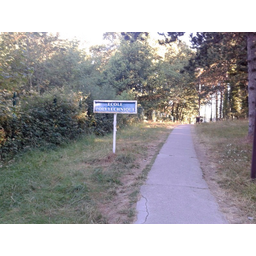
\includegraphics[width = 150pt]{Annexe/OursT.png}
     \caption{Image T}
      \end{minipage}\hfill
   \begin{minipage}{0.48\textwidth}
     \centering
     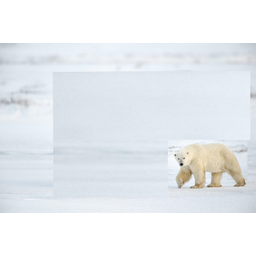
\includegraphics[width= 150pt]{Annexe/OursS.png}
     \caption{Image S}\label{Fig:Data2}
   \end{minipage}
\end{figure}

L'objectif est d'incruster toute ou partie de l'image S dans l'image T. En terme de manipulations, cela consiste à faire un mélange ou mixage des deux images, ou encore à effectuer un clonage lisse de la seconde image dans la première. Le résultat attendu pour une insertion "réussie" est un résultat comme celui présenté ci-dessous : 
    
\begin{center}
\begin{figure}[!htb]
   \centering
     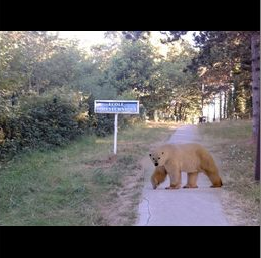
\includegraphics[width = 150pt]{Annexe/OursD.png}
     \caption{Image  finale attendue}
\end{figure}
\end{center}
Cette image a été obtenue à l'aide d'un de nos algorithmes, vous retrouvez les différents collage à la fin de ce rapport.\newline
\paragraph{Remarques}
Ce résultat semble naturel, les frontières entre l'image collée et l'arrière plan sont très peu visibles et ont été estompées, l'ours présent dans la première image n'a pas été déformé et semble faire parti de la photo initiale. 
Mais comment obtenir un tel résultat ?
\newline
En reprenant les deux images initiales, séparées, T et S et en effectuant un simple copier/coller, voici l'image que nous devrions obtenir : 
\begin{center}
\begin{figure}[H]
     \centering
     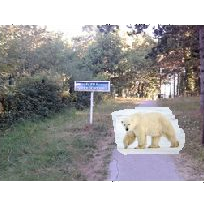
\includegraphics[width = 200pt]{beamIm/cccv.png}
     \caption{Simple copier/coller}
\end{figure}
\end{center}
Ici certains pixels de T, sont écrasés par ceux de l'image qui a été ajoutée. Ce résultat n'est bien entendu pas utilisable et bien loin de l'image finale attendue. Le découpage et le collage entre l'arrière-plan et l'image "objet" sont beaucoup trop visibles, les couleurs ne sont pas les mêmes et incohérentes. Le résultat doit être beaucoup plus naturel, comme écrit plus haut. Cette simple manipulation n'est donc pas suffisante pour effectuer le clonage cohérent  d'une image dans une autre. \newline

Il semble évident de vouloir modifier l'image finale obtenue ci-dessus afin qu'elle paraisse la plus naturelle possible.
Nous verrons tout au long de ce rapport, quels sont les changements à effectuer, et comment la résolution d'une équation aux dérivées partielles,l'équation de Poisson, permet d'obtenir un bien meilleur résultat. Nous implémenterons trois algorithmes permettant de résoudre le problème posé, et comparerons les résultats obtenus à l'aide de ceux-ci.
%%%%%%%%%%%%%%%%%%%%%%%%%%%%%%%%%%%%%%%%%%%%%%%%%%%%%%%%%%
%           TRADUCTION SOUS FORMES MATHEMATIQUES         %
%%%%%%%%%%%%%%%%%%%%%%%%%%%%%%%%%%%%%%%%%%%%%%%%%%%%%%%%%%

\subsection{Problème mathématique associé}

Comme écrit plus haut il faut apporter des modifications au précédent collage afin qu'il corresponde au mieux à nos attentes. En réalité nous ne souhaitons pas modifier l'entièreté de l'image mais seulement une "sous-image" correspondant à l'endroit du collage. Pour ce faire, considérons I, la partie de l'image finale à modifier. Il est ainsi possible de représenter le problème sous forme schématique. 
\begin{center}
    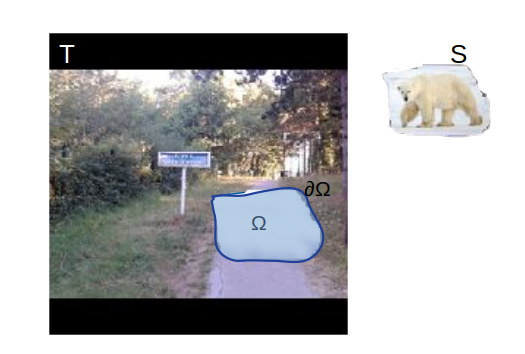
\includegraphics[width = 200pt]{beamIm/selectedscheme.png}
\end{center}

Avec : 
\begin{itemize}
    \item T,  l'image "Target", l'image destination, l'image sur laquelle s'effectuera le collage, l'arrière plan. 
    \item S, l'image "Source", l'image qui sera collée.
    \item $\Omega$, le domaine dans lequel se trouve l'inconnue.
    \item $\partial \Omega$, la frontière de $\Omega$.
    \item I, l'inconnue, la partie de l'image que nous ne connaissons pas et que nous voulons trouver, elle se situe dans $\Omega \cup \partial \Omega$
\end{itemize}

Nous souhaitons donc trouver une fonction I qui satisfasse un certain nombre de critères, afin de correspondre au résultat attendu.  
Cette fonction représente la partie modifiée de l'image. Mais quelles sont les conditions qu'elle doit remplir pour que le rendu soit le meilleur possible? Cette nouvelle image I doit-elle être plus proche de l'image collée S, ou de l'image d'arrière-plan T ? \newline

Pour que l'image obtenue s'incruste parfaitement, il faut que celle-ci dénature le moins possible les deux images sélectionnées au départ. En effet, les détails de l'image que nous voulons coller, S, doivent être retrouvés dans l'image finale, il ne faut donc pas modifier les variations qu'elle (S) pourrait posséder comme par exemple, les contours ou les objets lui appartenant. L'ours  à coller, doit être présent dans le collage final. Il faut donc être capable de retrouver dans l'image I, les informations présentes dans l'image initiale S. Par conséquent, il faut que les variations présentes dans $I$ soient presque identiques à celles de S.\\
Rappelons qu'en traitement d'image, les variations d'une image peuvent être obtenues en calculant son gradient. En effet, une variation peut être représentée comme un changement "brutal" d'intensité entre deux pixels. Le gradient d'une image étant numériquement obtenu en effectuant la différence entre des pixels voisins : si celle-ci est élevée alors il y a un fort changement d'intensité entre eux, (par exemple un pixel noir et un autre blanc), et donc possiblement la présence d'un contour. Par conséquent un gradient élevé détecte la présence de fortes variations. Au contraire, en l'absence de variations, le gradient est presque nul. Son calcul permet entre autre de détecter les contours d'une image.\\
Ici, il est nécessaire que les contours et objets de l'image finale soient très proches de ceux de l'image à coller. Mathématiquement, la fonction I possède donc un gradient, très proche(voir identique) à celui de l'image initiale S. Nous cherchons donc :
\begin{center}
    $$ min \iint_\Omega || \nabla I_{x,y} - \nabla S_{x,y}||^2 dxdy$$
\end{center} 

Mais les "frontières" entre l'image collée et l'image d'arrière-plan T, ne doivent pas non plus être visibles, il faut donc que les pixels se situant sur cette partie là, i.e $\partial \Omega$, soient le plus proches possible de T. En d'autres termes, les pixels de l'image finale sur le bord, coïncident avec ceux de l'image initiale T, au même endroit. La fonction I doit donc vérifier: 
\begin{center}
    $I_{(x,y)} = T_{x,y} \ sur\ \partial \Omega$
\end{center}

Répondre au problème implique donc de résoudre un problème variationnel classique auquel des conditions sur le bord de Dirichlet sont ajoutées. 
Voici donc le nouveau problème à résoudre :   

\begin{center}
\begin{equation}
\left\{
\begin{aligned}
 min \iint_\Omega || \nabla I_{x,y} - \nabla S_{x,y}||^2 dxdy\\
 I_{(x,y)} = T_{x,y} \ sur\ \partial \Omega
\end{aligned}
\right.
\end{equation}
\end{center}


\subsection{Résolution et équivalence avec l'équation de poisson}
Pour résoudre ce problème, il faut donc trouver le minimum de la fonction g suivante  : 
\begin{center}
\begin{equation}
\begin{aligned}
g(I) = \int_\Omega || \nabla I(x) - \nabla S(x)||^2 dx\\
\end{aligned}
\end{equation}
\end{center}
S'il existe alors celui-ci annule le gradient de la fonction. 
\subparagraph{Calcul de $\nabla g(I)$ }
En utilisant les formules de Taylor-Young à l'ordre 1, le gradient peut être calculé facilement :\\
Soit $u \in \mathbb{R}^n$, tel que $||u||=1$ :
\begin{equation*}
\begin{aligned}
g(I+\epsilon u) = g(I) +\epsilon \left<\nabla g(I), u\right> + o(\epsilon)\\
\end{aligned}
\end{equation*}
Posons : $v = \nabla S$.
\begin{equation*} 
\begin{aligned}
    g(I+\epsilon u) -g(I) =  \int_\Omega || \nabla (I+\epsilon u) - v||^2 - ||\nabla I -v ||^2 dx\\
\end{aligned}
\end{equation*} 
\begin{equation*} 
\left.
\begin{aligned}
    g(I+\epsilon u) -g(I) &=  \int_\Omega || \nabla I - v||^2+ ||\nabla \epsilon u||^2 +2(\nabla I - v)\times \epsilon \nabla u  - ||\nabla I -v ||^2 dx\\
  &=  \int_\Omega \epsilon ^2||\nabla u||^2 +2(\nabla I - v)\times \epsilon \nabla u dx\\
    & = 2\int_\Omega (\nabla I - v) \times (\nabla \epsilon u ) + O (\epsilon^2) \\ 
    & = 2\left<\nabla I - v, \nabla \epsilon u \right> + O (\epsilon^2) \\ 
      &  =   2\epsilon<\nabla I - v,  \nabla u> + O (\epsilon^2) \\ 
         &  = 2\left<\nabla I - v,  \nabla u \right> + O (\epsilon)\\ 
    & =  -2 <div(\nabla I - v), u > + O (\epsilon)\\
\end{aligned}
\right.
\end{equation*}
Par identification, le gradient de g vaut 
\begin{center}
		$\nabla g(I) = -2(\Delta I-div( v))$
\end{center} 
Le minimum de g annule son gradient, ainsi, si I est le minimum de la fonction alors il vérifie :
\begin{center}
		$0= (-\Delta I+div(v))$
\end{center}
\begin{center}
		$\Delta I =div(\nabla S)$\\
		$\Delta I = \Delta S$
		
\end{center} 

Trouver le minimum de (2) revient donc à résoudre l'équation : 
\begin{center}
$\Delta I = \Delta S$
\end{center}
Le nouveau problème est donc le suivant : 
\begin{center}
    \begin{equation}
        \left\{
        \begin{aligned}
         \Delta I = \Delta S  \ sur \  \Omega \\
          I = T \ sur \  \partial \Omega
        \end{aligned}
        \right.
    \end{equation}
\end{center}
Il n'est autre que l'équation de Poisson. Ainsi résoudre (1), est équivalent à résoudre l'équation de poisson avec conditions aux bords de Dirichlet. Nous décrirons dans ce rapport 3 manières de résoudre numériquement cette équation. 

